\documentclass{extbook}[14pt]
\usepackage{multicol, enumerate, enumitem, hyperref, color, soul, setspace, parskip, fancyhdr, amssymb, amsthm, amsmath, latexsym, units, mathtools}
\everymath{\displaystyle}
\usepackage[headsep=0.5cm,headheight=0cm, left=1 in,right= 1 in,top= 1 in,bottom= 1 in]{geometry}
\usepackage{dashrule}  % Package to use the command below to create lines between items
\newcommand{\litem}[1]{\item #1

\rule{\textwidth}{0.4pt}}
\pagestyle{fancy}
\lhead{}
\chead{Answer Key for Progress Quiz 7 Version A}
\rhead{}
\lfoot{3510-5252}
\cfoot{}
\rfoot{Summer C 2021}
\begin{document}
\textbf{This key should allow you to understand why you choose the option you did (beyond just getting a question right or wrong). \href{https://xronos.clas.ufl.edu/mac1105spring2020/courseDescriptionAndMisc/Exams/LearningFromResults}{More instructions on how to use this key can be found here}.}

\textbf{If you have a suggestion to make the keys better, \href{https://forms.gle/CZkbZmPbC9XALEE88}{please fill out the short survey here}.}

\textit{Note: This key is auto-generated and may contain issues and/or errors. The keys are reviewed after each exam to ensure grading is done accurately. If there are issues (like duplicate options), they are noted in the offline gradebook. The keys are a work-in-progress to give students as many resources to improve as possible.}

\rule{\textwidth}{0.4pt}

\begin{enumerate}\litem{
Construct the lowest-degree polynomial given the zeros below. Then, choose the intervals that contain the coefficients of the polynomial in the form $ax^3+bx^2+cx+d$.
\[ \frac{-4}{5}, \frac{-1}{2}, \text{ and } \frac{2}{5} \]The solution is \( 50x^{3} +45 x^{2} -6 x -8 \), which is option D.\begin{enumerate}[label=\Alph*.]
\item \( a \in [47, 51], b \in [44, 46], c \in [-10, -4], \text{ and } d \in [5, 10] \)

$50x^{3} +45 x^{2} -6 x + 8$, which corresponds to multiplying everything correctly except the constant term.
\item \( a \in [47, 51], b \in [-86, -79], c \in [41, 48], \text{ and } d \in [-11, -2] \)

$50x^{3} -85 x^{2} +46 x -8$, which corresponds to multiplying out $(5x -4)(2x -1)(5x -2)$.
\item \( a \in [47, 51], b \in [-50, -44], c \in [-10, -4], \text{ and } d \in [5, 10] \)

$50x^{3} -45 x^{2} -6 x + 8$, which corresponds to multiplying out $(5x -4)(2x -1)(5x + 2)$.
\item \( a \in [47, 51], b \in [44, 46], c \in [-10, -4], \text{ and } d \in [-11, -2] \)

* $50x^{3} +45 x^{2} -6 x -8$, which is the correct option.
\item \( a \in [47, 51], b \in [-35, -28], c \in [-16, -10], \text{ and } d \in [5, 10] \)

$50x^{3} -35 x^{2} -14 x + 8$, which corresponds to multiplying out $(5x -4)(2x + 1)(5x -2)$.
\end{enumerate}

\textbf{General Comment:} To construct the lowest-degree polynomial, you want to multiply out $(5x + 4)(2x + 1)(5x -2)$
}
\litem{
Describe the zero behavior of the zero $x = 4$ of the polynomial below.
\[ f(x) = -5(x + 4)^{6}(x - 4)^{7}(x + 5)^{3}(x - 5)^{6} \]The solution is the graph below, which is option A.
    \begin{center}
        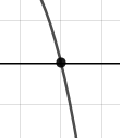
\includegraphics[width=0.3\textwidth]{../Figures/polyZeroBehaviorCopyAA.png}
    \end{center}\begin{enumerate}[label=\Alph*.]
\begin{multicols}{2}
\item 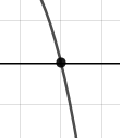
\includegraphics[width = 0.3\textwidth]{../Figures/polyZeroBehaviorCopyAA.png}
\item 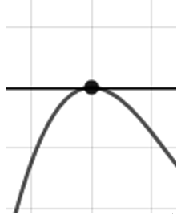
\includegraphics[width = 0.3\textwidth]{../Figures/polyZeroBehaviorCopyBA.png}
\item 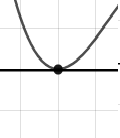
\includegraphics[width = 0.3\textwidth]{../Figures/polyZeroBehaviorCopyCA.png}
\item 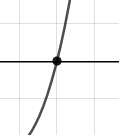
\includegraphics[width = 0.3\textwidth]{../Figures/polyZeroBehaviorCopyDA.png}
\end{multicols}\item None of the above.\end{enumerate}
\textbf{General Comment:} You will need to sketch the entire graph, then zoom in on the zero the question asks about.
}
\litem{
Which of the following equations \textit{could} be of the graph presented below?

\begin{center}
    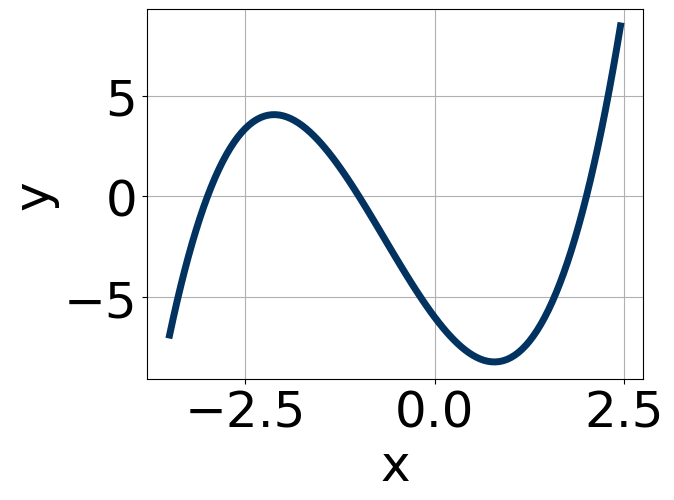
\includegraphics[width=0.5\textwidth]{../Figures/polyGraphToFunctionCopyA.png}
\end{center}


The solution is \( 15(x - 2)^{7} (x + 1)^{5} (x + 3)^{7} \), which is option C.\begin{enumerate}[label=\Alph*.]
\item \( 17(x - 2)^{8} (x + 1)^{9} (x + 3)^{11} \)

The factor $2$ should have been an odd power.
\item \( -7(x - 2)^{4} (x + 1)^{7} (x + 3)^{11} \)

The factor $(x - 2)$ should have an odd power and the leading coefficient should be the opposite sign.
\item \( 15(x - 2)^{7} (x + 1)^{5} (x + 3)^{7} \)

* This is the correct option.
\item \( -2(x - 2)^{11} (x + 1)^{9} (x + 3)^{9} \)

This corresponds to the leading coefficient being the opposite value than it should be.
\item \( 7(x - 2)^{10} (x + 1)^{8} (x + 3)^{11} \)

The factors $2$ and $-1$ have have been odd power.
\end{enumerate}

\textbf{General Comment:} General Comments: Draw the x-axis to determine which zeros are touching (and so have even multiplicity) or cross (and have odd multiplicity).
}
\litem{
Construct the lowest-degree polynomial given the zeros below. Then, choose the intervals that contain the coefficients of the polynomial in the form $x^3+bx^2+cx+d$.
\[ -4 - 2 i \text{ and } -1 \]The solution is \( x^{3} +9 x^{2} +28 x + 20 \), which is option B.\begin{enumerate}[label=\Alph*.]
\item \( b \in [0, 4], c \in [4.37, 5.42], \text{ and } d \in [2.7, 4.8] \)

$x^{3} + x^{2} +5 x + 4$, which corresponds to multiplying out $(x + 4)(x + 1)$.
\item \( b \in [6, 11], c \in [27.08, 28.41], \text{ and } d \in [14.4, 20.2] \)

* $x^{3} +9 x^{2} +28 x + 20$, which is the correct option.
\item \( b \in [-9, -7], c \in [27.08, 28.41], \text{ and } d \in [-20.3, -18.9] \)

$x^{3} -9 x^{2} +28 x -20$, which corresponds to multiplying out $(x-(-4 - 2 i))(x-(-4 + 2 i))(x -1)$.
\item \( b \in [0, 4], c \in [0.79, 4.62], \text{ and } d \in [-0.4, 3.2] \)

$x^{3} + x^{2} +3 x + 2$, which corresponds to multiplying out $(x + 2)(x + 1)$.
\item \( \text{None of the above.} \)

This corresponds to making an unanticipated error or not understanding how to use nonreal complex numbers to create the lowest-degree polynomial. If you chose this and are not sure what you did wrong, please contact the coordinator for help.
\end{enumerate}

\textbf{General Comment:} Remember that the conjugate of $a+bi$ is $a-bi$. Since these zeros always come in pairs, we need to multiply out $(x-(-4 - 2 i))(x-(-4 + 2 i))(x-(-1))$.
}
\litem{
Which of the following equations \textit{could} be of the graph presented below?

\begin{center}
    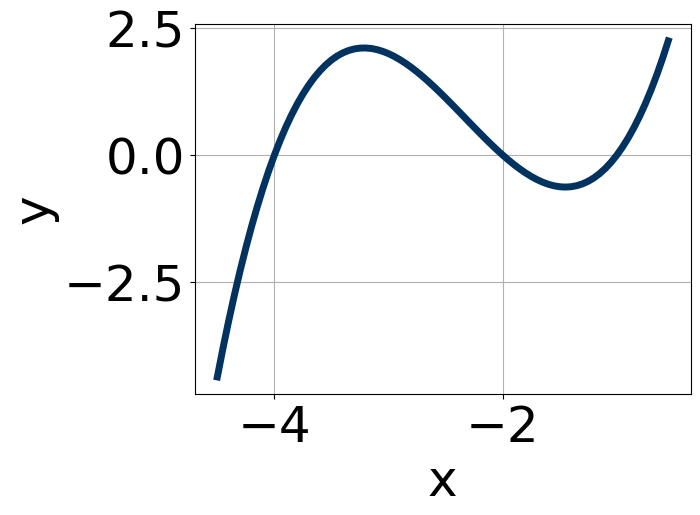
\includegraphics[width=0.5\textwidth]{../Figures/polyGraphToFunctionA.png}
\end{center}


The solution is \( 9(x + 1)^{9} (x + 2)^{7} (x + 4)^{11} \), which is option C.\begin{enumerate}[label=\Alph*.]
\item \( -7(x + 1)^{5} (x + 2)^{9} (x + 4)^{9} \)

This corresponds to the leading coefficient being the opposite value than it should be.
\item \( 10(x + 1)^{10} (x + 2)^{5} (x + 4)^{7} \)

The factor $-1$ should have been an odd power.
\item \( 9(x + 1)^{9} (x + 2)^{7} (x + 4)^{11} \)

* This is the correct option.
\item \( -2(x + 1)^{10} (x + 2)^{5} (x + 4)^{5} \)

The factor $(x + 1)$ should have an odd power and the leading coefficient should be the opposite sign.
\item \( 20(x + 1)^{10} (x + 2)^{8} (x + 4)^{9} \)

The factors $-1$ and $-2$ have have been odd power.
\end{enumerate}

\textbf{General Comment:} General Comments: Draw the x-axis to determine which zeros are touching (and so have even multiplicity) or cross (and have odd multiplicity).
}
\litem{
Describe the zero behavior of the zero $x = 3$ of the polynomial below.
\[ f(x) = 6(x + 5)^{4}(x - 5)^{2}(x + 3)^{13}(x - 3)^{8} \]The solution is the graph below, which is option C.
    \begin{center}
        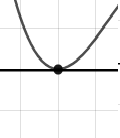
\includegraphics[width=0.3\textwidth]{../Figures/polyZeroBehaviorCA.png}
    \end{center}\begin{enumerate}[label=\Alph*.]
\begin{multicols}{2}
\item 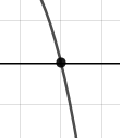
\includegraphics[width = 0.3\textwidth]{../Figures/polyZeroBehaviorAA.png}
\item 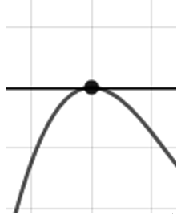
\includegraphics[width = 0.3\textwidth]{../Figures/polyZeroBehaviorBA.png}
\item 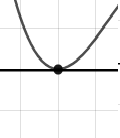
\includegraphics[width = 0.3\textwidth]{../Figures/polyZeroBehaviorCA.png}
\item 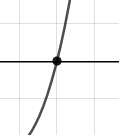
\includegraphics[width = 0.3\textwidth]{../Figures/polyZeroBehaviorDA.png}
\end{multicols}\item None of the above.\end{enumerate}
\textbf{General Comment:} You will need to sketch the entire graph, then zoom in on the zero the question asks about.
}
\litem{
Describe the end behavior of the polynomial below.
\[ f(x) = -9(x - 5)^{3}(x + 5)^{8}(x - 6)^{4}(x + 6)^{6} \]The solution is the graph below, which is option A.
    \begin{center}
        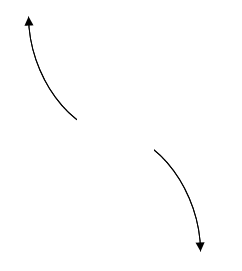
\includegraphics[width=0.3\textwidth]{../Figures/polyEndBehaviorAA.png}
    \end{center}\begin{enumerate}[label=\Alph*.]
\begin{multicols}{2}
\item 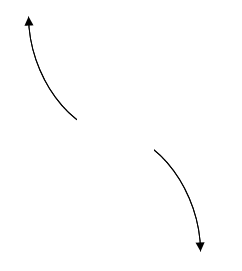
\includegraphics[width = 0.3\textwidth]{../Figures/polyEndBehaviorAA.png}
\item 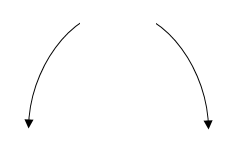
\includegraphics[width = 0.3\textwidth]{../Figures/polyEndBehaviorBA.png}
\item 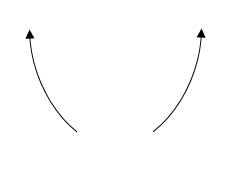
\includegraphics[width = 0.3\textwidth]{../Figures/polyEndBehaviorCA.png}
\item 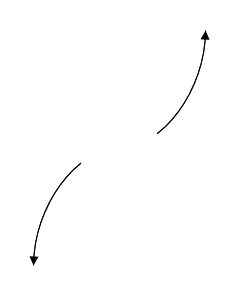
\includegraphics[width = 0.3\textwidth]{../Figures/polyEndBehaviorDA.png}
\end{multicols}\item None of the above.\end{enumerate}
\textbf{General Comment:} Remember that end behavior is determined by the leading coefficient AND whether the \textbf{sum} of the multiplicities is positive or negative.
}
\litem{
Describe the end behavior of the polynomial below.
\[ f(x) = 2(x + 2)^{2}(x - 2)^{7}(x + 8)^{4}(x - 8)^{4} \]The solution is the graph below, which is option D.
    \begin{center}
        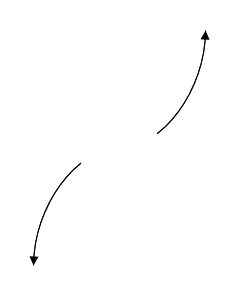
\includegraphics[width=0.3\textwidth]{../Figures/polyEndBehaviorCopyDA.png}
    \end{center}\begin{enumerate}[label=\Alph*.]
\begin{multicols}{2}
\item 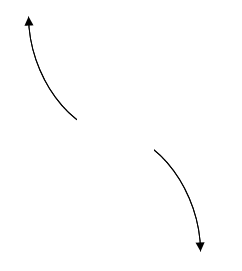
\includegraphics[width = 0.3\textwidth]{../Figures/polyEndBehaviorCopyAA.png}
\item 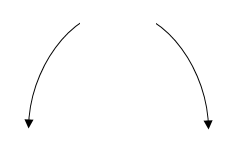
\includegraphics[width = 0.3\textwidth]{../Figures/polyEndBehaviorCopyBA.png}
\item 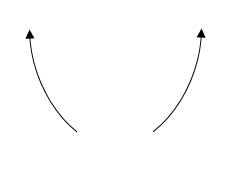
\includegraphics[width = 0.3\textwidth]{../Figures/polyEndBehaviorCopyCA.png}
\item 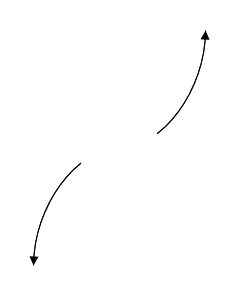
\includegraphics[width = 0.3\textwidth]{../Figures/polyEndBehaviorCopyDA.png}
\end{multicols}\item None of the above.\end{enumerate}
\textbf{General Comment:} Remember that end behavior is determined by the leading coefficient AND whether the \textbf{sum} of the multiplicities is positive or negative.
}
\litem{
Construct the lowest-degree polynomial given the zeros below. Then, choose the intervals that contain the coefficients of the polynomial in the form $ax^3+bx^2+cx+d$.
\[ \frac{4}{3}, \frac{7}{5}, \text{ and } \frac{-1}{3} \]The solution is \( 45x^{3} -108 x^{2} +43 x + 28 \), which is option D.\begin{enumerate}[label=\Alph*.]
\item \( a \in [44, 48], b \in [-108, -105], c \in [40, 50], \text{ and } d \in [-28, -27] \)

$45x^{3} -108 x^{2} +43 x -28$, which corresponds to multiplying everything correctly except the constant term.
\item \( a \in [44, 48], b \in [9, 14], c \in [-86, -82], \text{ and } d \in [-28, -27] \)

$45x^{3} +12 x^{2} -85 x -28$, which corresponds to multiplying out $(3x + 4)(5x -7)(3x + 1)$.
\item \( a \in [44, 48], b \in [127, 141], c \in [121, 128], \text{ and } d \in [25, 34] \)

$45x^{3} +138 x^{2} +125 x + 28$, which corresponds to multiplying out $(3x + 4)(5x + 7)(3x + 1)$.
\item \( a \in [44, 48], b \in [-108, -105], c \in [40, 50], \text{ and } d \in [25, 34] \)

* $45x^{3} -108 x^{2} +43 x + 28$, which is the correct option.
\item \( a \in [44, 48], b \in [107, 110], c \in [40, 50], \text{ and } d \in [-28, -27] \)

$45x^{3} +108 x^{2} +43 x -28$, which corresponds to multiplying out $(3x + 4)(5x + 7)(3x -1)$.
\end{enumerate}

\textbf{General Comment:} To construct the lowest-degree polynomial, you want to multiply out $(3x -4)(5x -7)(3x + 1)$
}
\litem{
Construct the lowest-degree polynomial given the zeros below. Then, choose the intervals that contain the coefficients of the polynomial in the form $x^3+bx^2+cx+d$.
\[ -5 - 3 i \text{ and } 1 \]The solution is \( x^{3} +9 x^{2} +24 x -34 \), which is option A.\begin{enumerate}[label=\Alph*.]
\item \( b \in [4, 14], c \in [23.5, 25.2], \text{ and } d \in [-34.6, -33] \)

* $x^{3} +9 x^{2} +24 x -34$, which is the correct option.
\item \( b \in [-5, 6], c \in [3.8, 6.7], \text{ and } d \in [-6.8, -4] \)

$x^{3} + x^{2} +4 x -5$, which corresponds to multiplying out $(x + 5)(x -1)$.
\item \( b \in [-10, -2], c \in [23.5, 25.2], \text{ and } d \in [33.9, 36.6] \)

$x^{3} -9 x^{2} +24 x + 34$, which corresponds to multiplying out $(x-(-5 - 3 i))(x-(-5 + 3 i))(x + 1)$.
\item \( b \in [-5, 6], c \in [-1.7, 3.3], \text{ and } d \in [-3.6, -0.7] \)

$x^{3} + x^{2} +2 x -3$, which corresponds to multiplying out $(x + 3)(x -1)$.
\item \( \text{None of the above.} \)

This corresponds to making an unanticipated error or not understanding how to use nonreal complex numbers to create the lowest-degree polynomial. If you chose this and are not sure what you did wrong, please contact the coordinator for help.
\end{enumerate}

\textbf{General Comment:} Remember that the conjugate of $a+bi$ is $a-bi$. Since these zeros always come in pairs, we need to multiply out $(x-(-5 - 3 i))(x-(-5 + 3 i))(x-(1))$.
}
\end{enumerate}

\end{document}